\newpage
\section{Projektplanung}

\subsection{Risikobewertung}

Alle bekannten Risiken von dem Projekt sind in folgenden Tabelle aufgelistet.
Dabei hat jedes Risiko folgende Attribute:
\begin{itemize}
    \item \textbf{Titel + Beschreibung}: Beschreibung des Risikos
    \item \textbf{Verantwortlich} Welche Gruppe dafür Verwantwortlich ist (INF=Informatik, MT=Mechaniker, ET=Elektroniker).
    \item \textbf{Kategorie}: In welcher Kategorie sich das Risiko befindet.
    \item \textbf{Ursachen}: Was passieren muss, damit das Risiko eintreffen kann.
    \item \textbf{Bewertung des Risikos}: Eintrittswahrscheinlichkeit, Auswirkung und Risiko Bewertung ohne Massnahmen
    \item \textbf{Massnahmen zur Risikominimierung}: Massnahmen um die Eintrittswahrscheinlichkeit oder Auswirkung zu minimieren.
    \item \textbf{Korrekturmassnahmen}: Was gemacht werden soll, wenn das Risiko trotzdem Eintrifft
    \item \textbf{Erfolgsfaktoren}: Beschreibt das Verhalten bei erfolgreicher Risikomitigation
    \item \textbf{Erneute Bewertung des Risikos}: Eintrittswahrscheinlichkeit, Auswirkung und Risiko Bewertung mit den definierten Massnahmen
\end{itemize}
\begin{landscape}
\scriptsize
\begin{longtable}{|c|p{4cm}|p{4cm}|c|c|p{4cm}|c|c|c|p{4cm}|p{4cm}|p{4cm}|c|c|c|}
\hline
ID & Title & Description & Ver. & Kategorie & Ursachen &  & Impact & Risk Score & Preventive Measure & Corrective Measure (Was, wenn trotzdem eintritt?) & Success Factors & Probability ' & Impact ' & Risk Score ' \\
\hline
R1 & Grip-Verlust normale Räder & Das Fahrzeug schleift über den Boden & MT & Mechanisch & Fahrzeug verliert Grip & Possible & Moderate & 9 & Auf Mensaboden testen & Andere Räder/Geschwindigkeit anpassen & Fahrzeug hat Grip & Unlikely & Minor & 4 \\
\hline
R2 & Liniensensor falsche Daten & Der Liniensensor erkennt die Fugen als Führungslinie & ET+INF & Elektrisch & Fahrzeug folgt der Fuge & Likely & Major & 16 & Kalibrierung des Sensors, Abgleich mit Kamera. Befahren einer Linie nur, wenn Punkt oder Hindernis am Ende erkannt & Not-Aus verwenden & Fahrzeug folgt Führungslinie & Unlikely & Critical & 10 \\
\hline
\end{longtable}
\normalsize
\end{landscape}


\addtocounter{subsection}{1}
\addcontentsline{toc}{subsection}{ TODO.1   Projektplan}
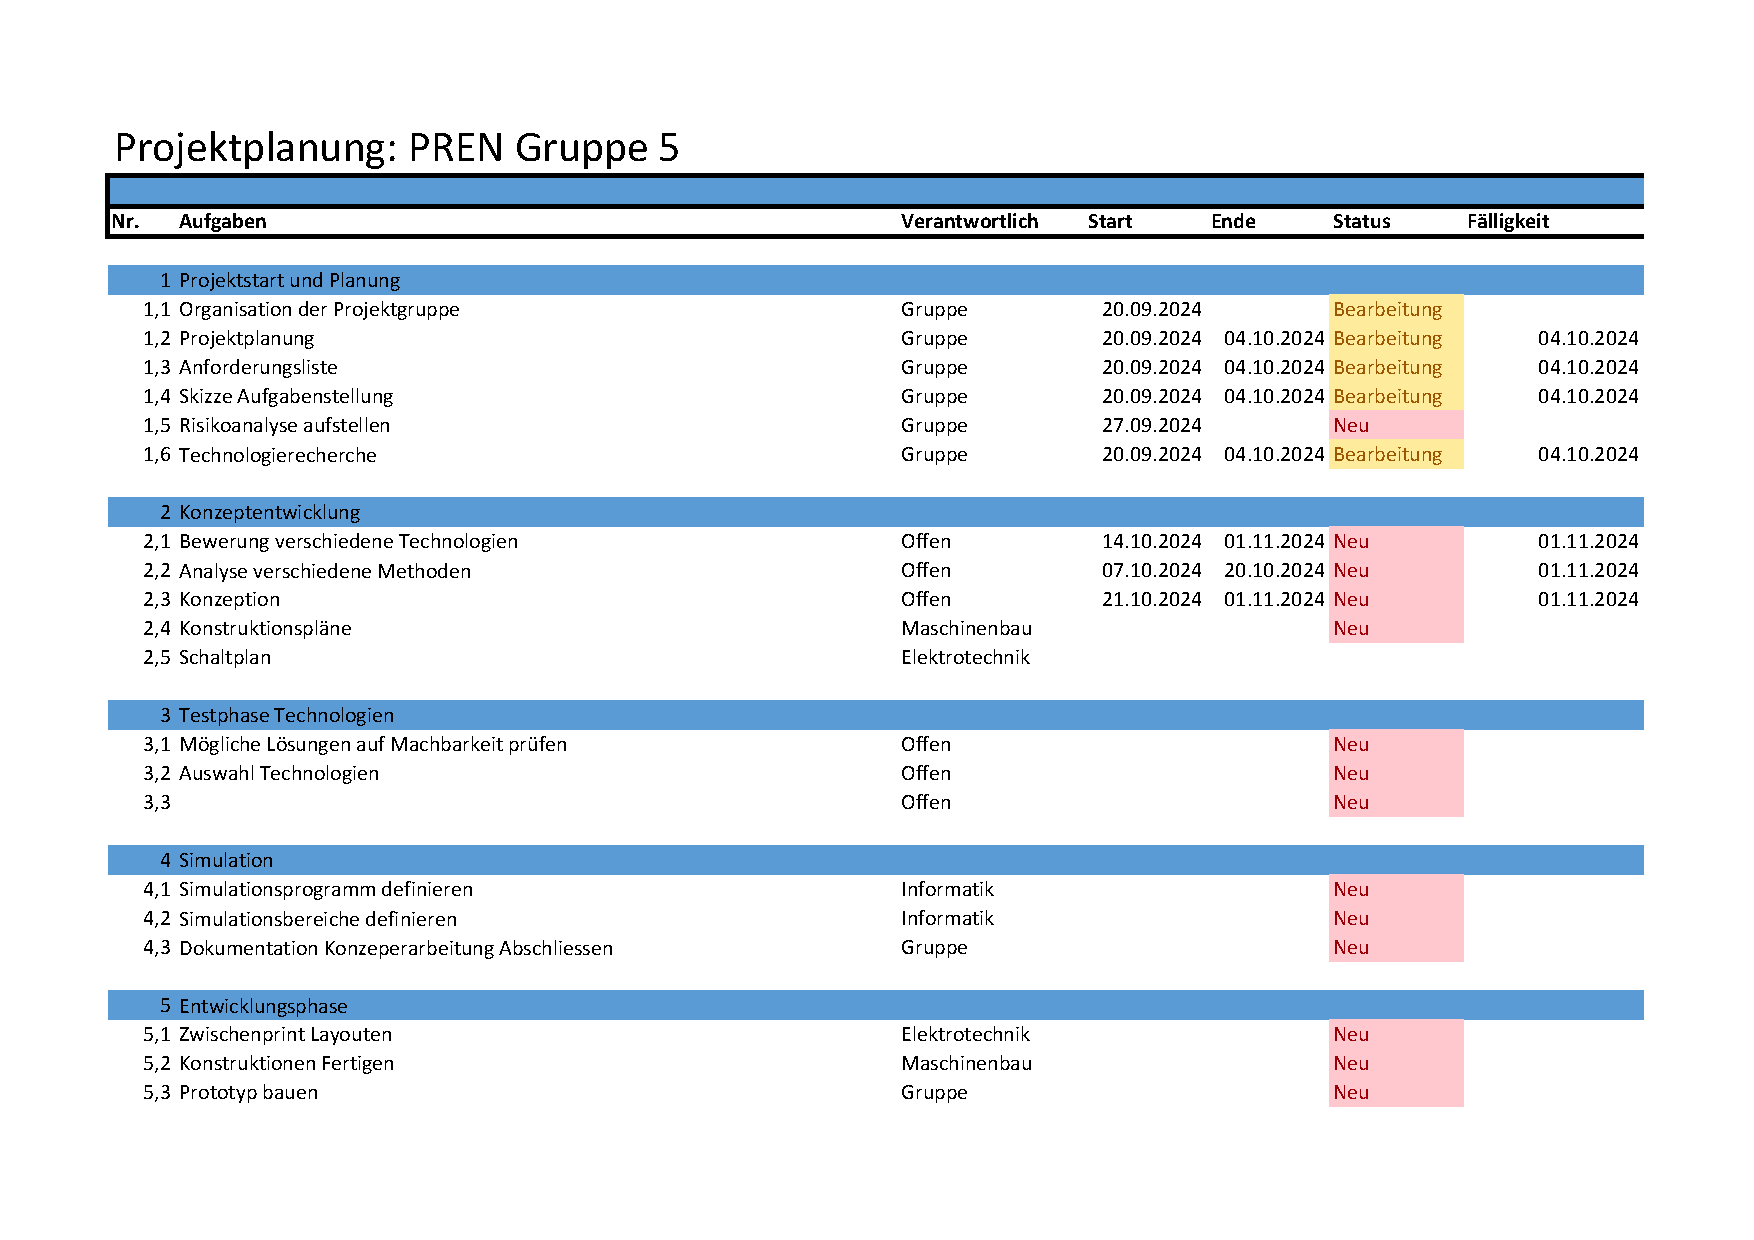
\includepdf[
  landscape=true,
  pages={1-},
  scale=0.9,
  pagecommand={\pagestyle{fancy}}
]{assets/Projektplan.pdf}

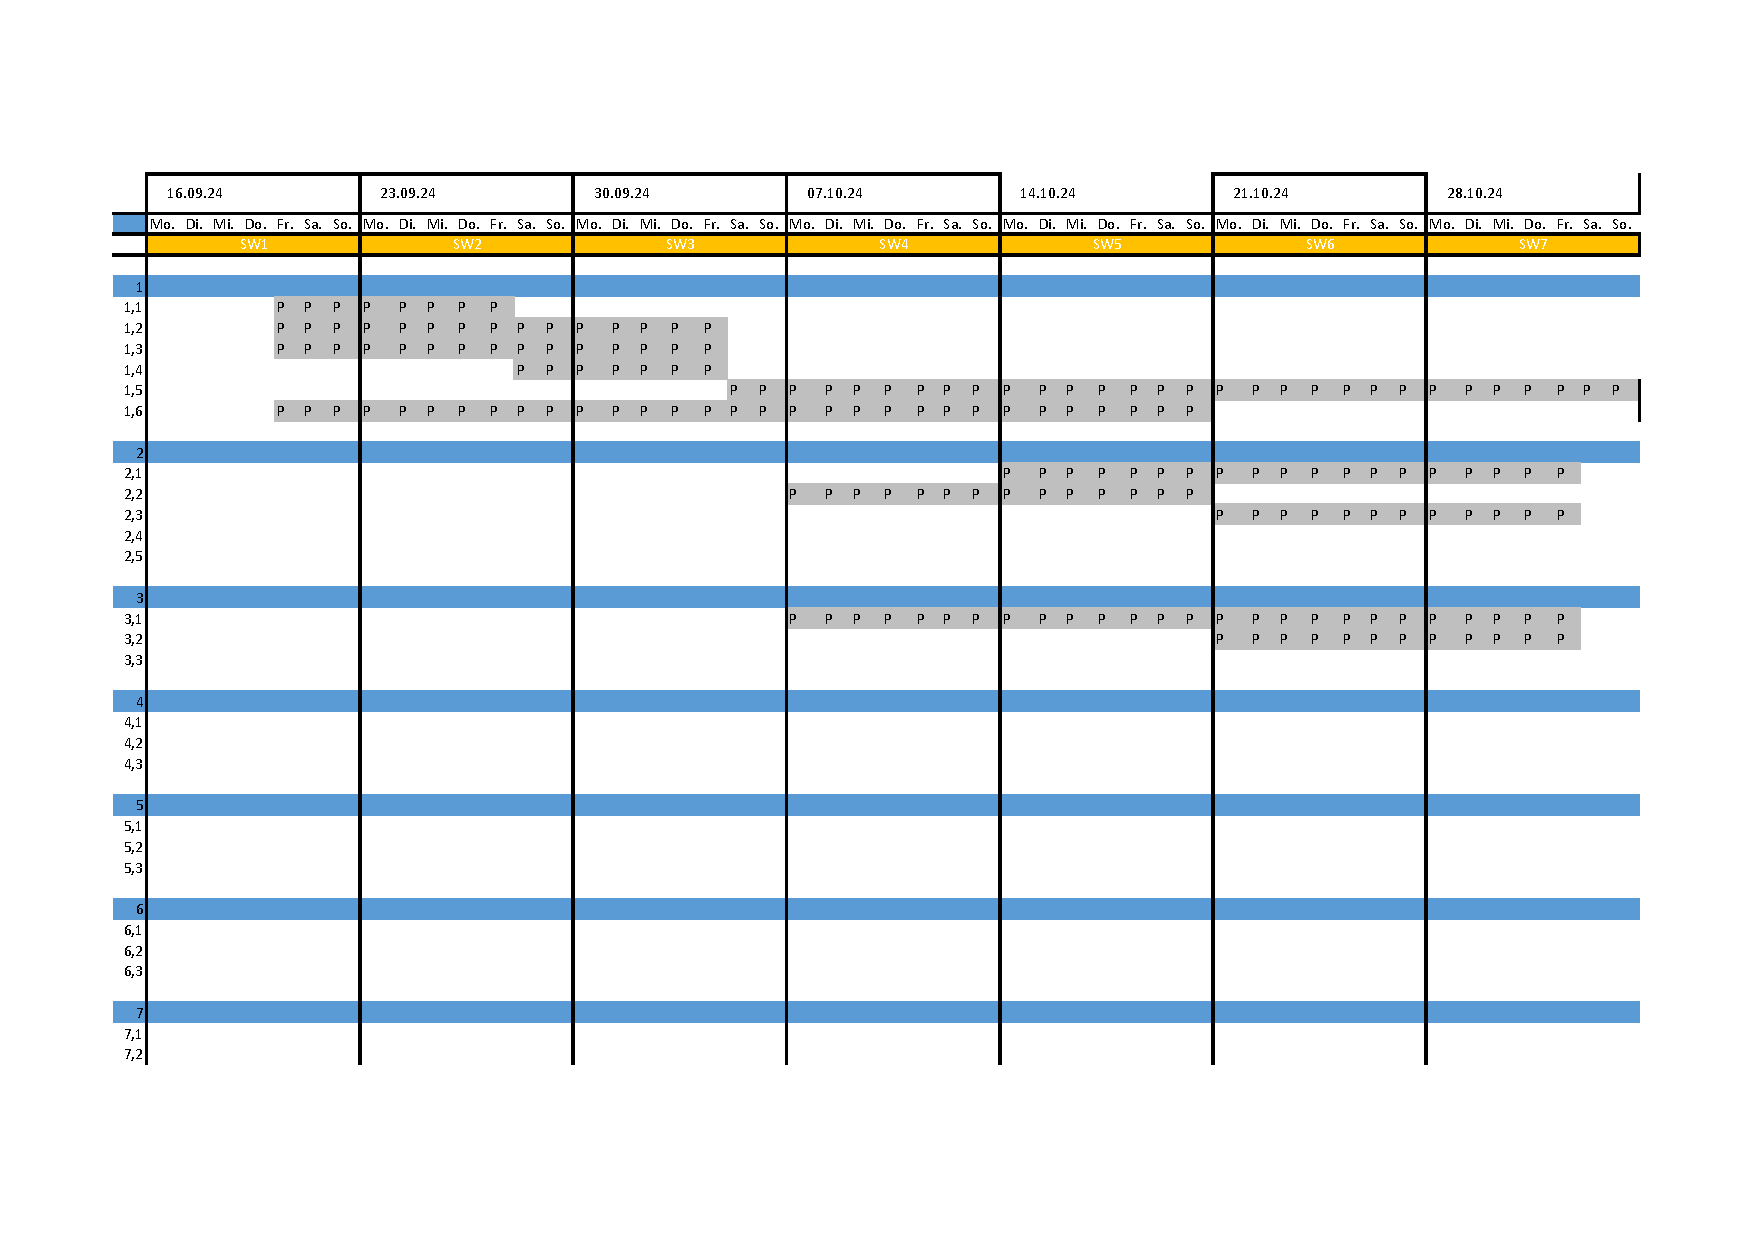
\includepdf[
  landscape=true,
  pages={1-},
  scale=0.9,
  pagecommand={\pagestyle{fancy}}
]{assets/Zeitplan.pdf}
